\documentclass{article}
\usepackage[utf8]{inputenc}
\usepackage{natbib}
\usepackage{url}
\usepackage{graphicx}
\usepackage{caption}
\usepackage[a4paper, margin=1.0cm]{geometry}

\title{
    Synthetic Data for a Model Based Learning System
}

\author{Sonke Wohler \\
\begin{small}
    s.wohler.15@aberdeen.ac.uk
\end{small}
}
\date{\begin{small}\today\end{small}}

\pagestyle{empty}

%\bibliographystyle{unsrt}
%\bibliographystyle{abbrv}
\bibliographystyle{plain}
%\bibliographystyle{apalike}

%********************************************************************************

\begin{document}


\thispagestyle{empty}

\begin{center}
\begin{LARGE}Synthetic Data for a Model Based Learning System\end{LARGE}
\bigskip
\bigskip
\\\begin{Large}Sonke Wohler\end{Large}
\\\begin{large}s.wohler.15@aberdeen.ac.uk\end{large}
\bigskip
\smallskip
\\\begin{large}A Joint Honours Project Plan\end{large}
\smallskip
\\From the Department of Computing Science
\\ And the Department of Physics
\medskip
\\University of Aberdeen
\bigskip
\smallskip
\\Supervised by Dr Ernesto Compatangelo
\medskip
\\Time frame: Jan -May 2019
\end{center}
\clearpage

\section{Context of the Project}


As with many Industries Oil and Gas is beginning to understand the value of Data and Data Analysis. \textsuperscript{\cite{chickenEgg,cloudOil}}
One possible product of Data Analysis is a suitable Mathematical Model that would describe the Real World Phenomena and allow predictions about how these phenomena might play out and that would allow them to draw more sophisticated conclusions from Data. 
Even where no additional knowledge can be gained from a Model it can improve the automation prospects for certain analysis tasks while guaranteeing transparency to the Engineers already working in the business and on the relevant projects. This sets Mathematical Models apart from other automation techniques where the inner workings of the automation are often rather opaque especially to non-Programmers. 
\\\\()
One such phenomenon for example are the sounds that can be recorded in deep sea wells, originating at the Oil Reservoirs underground. Analysis of this Data, currently carried out by human analysts, can reveal information about the reservoirs and some processes they might be going through.
\\ As with many tasks, the prospect of automating this analysis may provide significant improvements, at the least by reducing cost.
()
  \subsection{Synthetic Data}
  
Once a Model is defined it can be used to produce Synthetic Data by creating an Emulator. This Data can be used as a prediction to compare to Real Data of the Phenomenon that is to be studied. The accuracy of the prediction allows deductions about the accuracy of the Model, which in turn can be adapted and improved based on these.
\\\\ This process is a variation of Mathematical Modelling which forms the basis of much scientific research, in particular in the field of Physics, which it is closely associated with, but has become more common in almost any research field in recent decades, and perhaps even more so in business research.   \textsuperscript{\cite{modelling}}

  \begin{figure}[h]
    \centering
    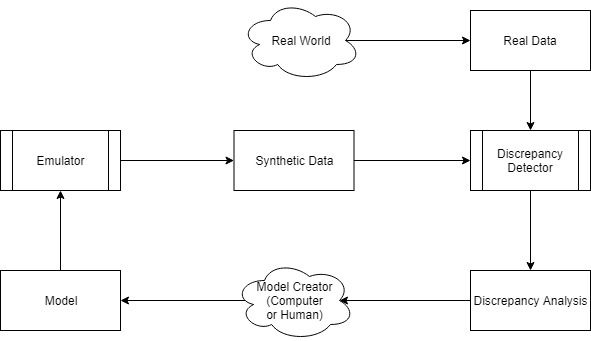
\includegraphics[width=0.7\linewidth]{figures/ModelLearning}
    \caption{A Schematic of Model Based Machine Learning}The Synthetic Data produced by the Emulator is compared against Real Data and the resulting Discreptancy Analysis informs the Model Creator in the adaptation of the Mathematical Model. Note that creating and adapting the Model is currently a Human Task, but even automation in all but this aspect may present an improvement in effectiveness of the Process.
    \label{fig:modelLearning}
\end{figure}
  
  \subsection{Model Based Machine Learning}
  
Given the clearly defined nature of the above described Process, its automation would present an interesting prospect, as well as the potential downsides and limitations to this Technology.
\\ Figure \ref{fig:modelLearning} describes a possible set up that could facilitate such automation, which may well be called Model Based (Machine) Learning. It would require an Emulator that can provide Synthetic Data based on a Model, which is currently for the most part programmed on demand by somebody with scientific programming expertise around a defined Model. 

  

\section{The Project}

The conceptual challenge to this project shall be the Concept of Model Based Machine Learning and what can be learned about its principles and limitations.
\\ Within this Concept the Emulator Module is likely the best starting point, given the relative familiarity of scientific programming. The novelty to an emulator in such a Machine Learning set up is that it cannot be build around one particular Model for a specific phenomenon. Instead it must produce an accurate Dataset based on whatever Model it is provided with, and must provide functionality for defining such a Model. This is unlike existing Emulators that are largely optimised and constrained to their particular application, and that do not allow meaningful adaptations to the Model without programmatic alterations.

  \subsection{Requirement Specifications}
  
The Student is aiming to fulfil the following Software Development Goals:

    \begin{enumerate}
      \item (Must Have) An Emulator Module that produces a set of synthetic data based on a defined, mathematical Model.
      \item (Must Have) The Emulator will offer some means for a user to define and change said Model Mathematically.
      \item (Should Have) The Emulator may provide some means for a user to define the nature of the dataset that is produced.
      \item (Should Have) The Mathematical Model definition when carried out by the user should be as user friendly as possible without compromising the Emulator's capabilities, and not require Programming experience or access.
      \item (Should Have) Sufficient and quality documentation of said Emulator to allow further development and refactoring as well as quality-assessment.
      \item (Could Have) Investigation into the capabilities and limitations of Model Based Machine Learning
      \item (Won't Have) Investigation to aid the Design of further Prototypes complementing the above Module in automating Mathematical Modelling Processes.
      \item (Won't Have) The Emulator may provide support to the user in homogenising and comparing the synthetic data to some set of real data provided by the user.
    \end{enumerate}

  \subsection{Proposed Project Time-line}

    \begin{figure}[h]
      \centering
      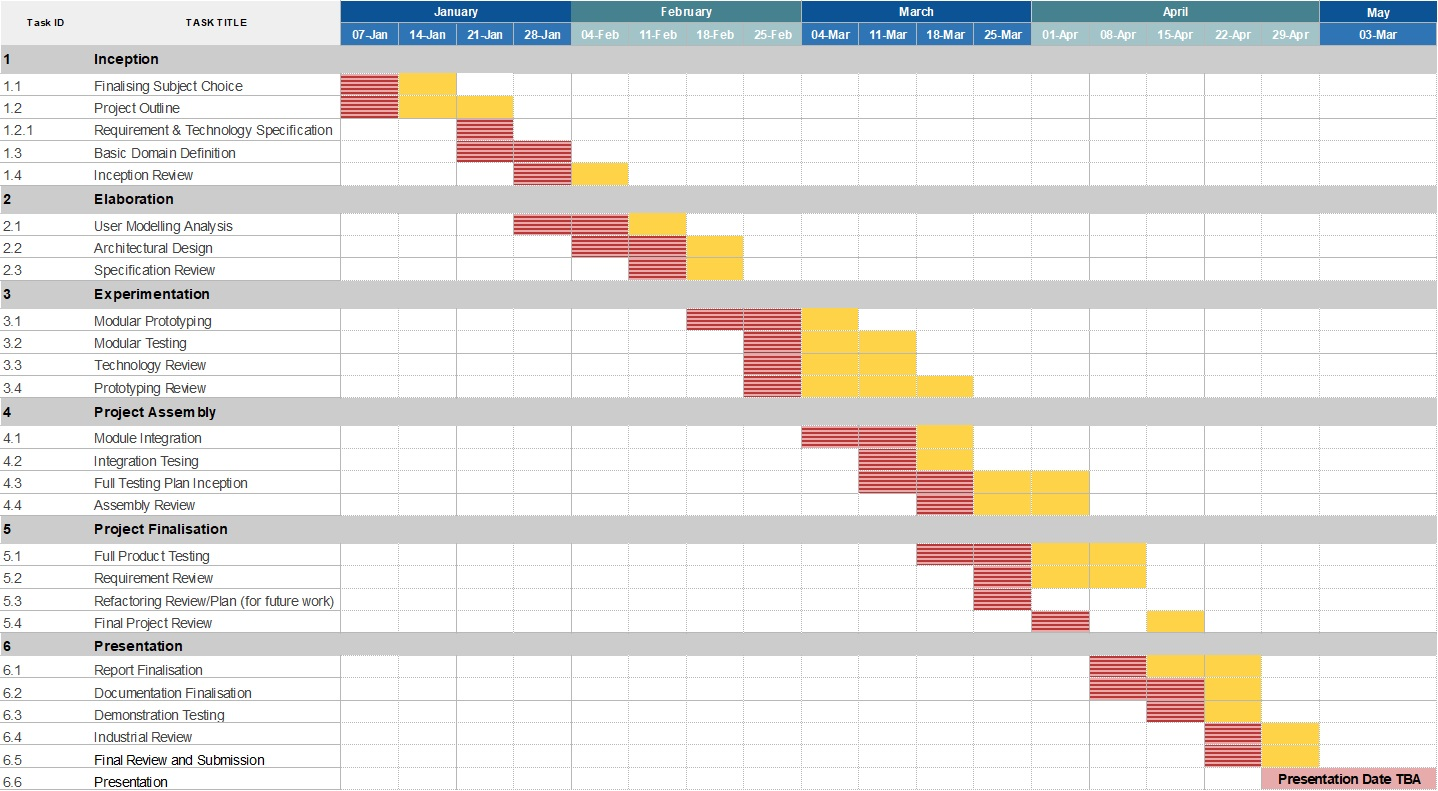
\includegraphics[width=\linewidth]{figures/ProjectPlan.jpg}
      \caption{Gantt Chart of a time-line that aims to deliver on the above specified goals, with best case time-line in pink and worst case time-line in orange.
      }
      \label{fig:gantt}
    \end{figure}

  \subsection{Risk Factors and Other Considerations}

Project will be related to a concrete application for which Clients will be providing Data. However as he goal is a general Emulator that is not specific to a particular application this should not break the project, but would simply slow it down. The availability of a Dataset would be preferable as it provides concrete examples and Test Cases that support debugging and Development.
  









\clearpage
\bibliography{refs}

\end{document}
